\section{Genetische Algorithmen}

% Was ist n Genetischer Algorithmus
Genetische Algorithmen nehmen Inspiration von der Evolutionstheorie von Charles Darwin
Dass angepasstere Individuen erfolgreicher darin sind ihre Genetischen Informationen zu verbreiten

Die zugrundeliegenden Idee ist, dass angepasstere Individuen eine 
höhere Chance haben Nachkommen zu erzeugen. \cite*{GeneticAlgorithms}

Wie die meißten stochastischen Algorithmen haben genetische Algorithmen keine 
Garantie ein globales Optimum zu finden \cite*{GeneticAlgorithms}


Das besonderen an genetischen Algorithmen ist, dass diese nicht mit Werten aus dem
Suchraum des Problems selbst arbeiten, sondern mit Chromosomrepresentationen.~\cite*{TerminologiesAndOperators}
Ein Chromosom ist also eine Vektorrepresentation einer Lösung aus dem Suchraum.
Die einzelnen Werte eines Chromosoms nennt man Gene und eine Menge an Genen 
bilden eine Population. [Siehe Grafik 01]
Die Chromosomrepresentation kann Binär, Hexadezimal, mit Fließkommazahlen oder auch anderen Symbolen geschehen.
Welche Werte die Gene einnehmen können hängt von der Problemdomäne ab.

% DO: Grafik Population, Gen, Individual
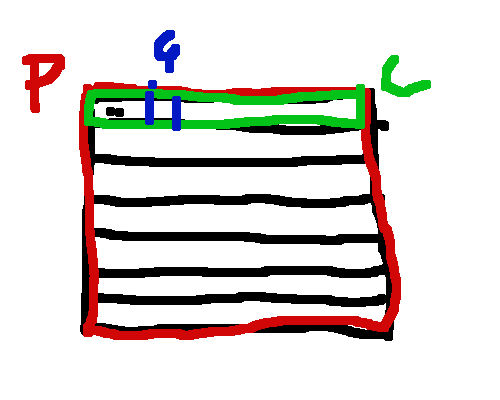
\includegraphics[scale=1.0]{images/Population_Chromosom_Gen.png}


% Key Components
Die Hauptbestandteile eines Genetischen Algorithmus, welche von jeder Variante implementiert werden
sind Representationsoperator, Fitnessfunktion und genetische Operatoren.

Der Representationsoperator übersetzt eine Lösung aus dem Suchraum in eine Chromosomrepresentation.

Die Fitnessfunktion einem gegebenen Chromosom einen Fitnesswert zu, anhand welcher
die Chromosome verglichen werden können. Die Fitness eines Chromosoms entspricht 
dem Wert der objektiven Funktion an der Stelle welche das Chromosom representiert.~\cite*{TerminologiesAndOperators}

Die genetischen Operatoren sind aufgeteilt in Selektionsoperator, Mutationsoperator und
Crossoveroperator. Im folgenden werde ich die einzelnen Operatoren erläutern und 
beliebte Implementationen aufführen. 

\subsection{Selektionsoperator}
Der Selektionsoperator wählt eine Menge von Eltern aus der Population, aus 
welchen Kinder für die nächste Generation erzeugt werden.
Typischerweise hat jedes Kind-Chromosom zwei Eltern-Chromosome. Es gibt jedoch auch 
Crossover-Operatoren welche mit mehr als zwei Eltern arbeiten.
Ganz nach der Evolutionstheorie sollen hier Chromosome mit einer höheren Fitness
auch eine höhere Chance haben als Elternteil gewählt zu werden.
Wie stark Chromosome mit einer höheren Fitness bevorzugt werden wird als Selektionsdruck bezeichnet.
Selektionsschemata können in zwei Klassen unterteilt werden, proportionale Selektion 
und ordinale Selektion.~\cite*{TerminologiesAndOperators} Eine proportionale Selektion gewichtet Chromosome anhand ihrer Fitness.
Ordinale Selektion gewichtet Chromosome anhand ihres Ranges.
Der Selektionsdruck
Bei einer proportionalen Selektion ist der Selektionsdruck hoch und es besteht das Risiko einer verfrühten Konvergenz.
Denn wenn es ein Chromosom gibt, welches weitaus fitter als der Rest der Population ist 
wird dieses einen proportionalen Selektionsprozess dominieren und somit die genetische 
Diversität der Population senken.
Andererseits führt ein geringer Selektionsdruck zu langsamer konvergenz.~\cite*{TerminologiesAndOperators}
Die Auswahl des Selektionsoperators sollte also wohlüberdacht sein.

\subsubsection*{Roulette Rad Selektion}
Roulette Rad Selektion ist einer der traditionellen proportionalen Selektionsoperatoren.
Stellen wir uns ein Roulette Rad vor, welches in $N$ Segmente unterteilt ist, 
wobei $N$ die Anzahl der Chromosome in einer Population ist.
Die Länge eines Segmentes $s_i$ ist proportional zu der normalisierten Fitness des korrespondierenden Chromosoms.
\begin{equation}
    s_i = 2 \pi \cdot \frac{fitness(i)}{\sum_{j=1}^{N} fitness(j)}
\end{equation}
Nun wird das Roulette Rad gedreht und das Chromosom auf wessen Feld man landet wird
in die Menge der Eltern aufgenommen.
Diese Prozedur wird so oft wiederholt bis man die gewünschte Anzahl an Eltern gesammelt hat.

\subsubsection*{Zufällige Selektion}
Der zufällige Selektionsoperator ist der simpelste.
Jedes Chromosom hat die gleiche Wahrscheinlichkeit in die Elternmenge aufgenommen zu werden.

\subsubsection*{Rang Selektion}
Die Rang Selektion ist eine Abwandlung der Roulette Rad Selektion.
Die länge eines Segmentes ist jedoch nicht proportional zu der fitness sondern proportional zu dem Rang des Chromosoms.
\begin{equation}
    s_i = 2 \pi \cdot \frac{N - rank(i)}{\sum_{j=1}^{N} rank(j)}
\end{equation}

\subsubsection*{Elitismus}
Die Selektionsoperatoren garantieren nicht, dass die besten Chromosome ausgewählt werden.
Darüber hinaus kann es vorkommen, dass die besten Chromosome durch Crossover und Mutation verschlechtert werden,
sodass die Fitness der folgenden Generation geringer als die vorherige ist.
Um eine Abnahme der Fitness zu verhindern kann wird Elitismus angewendet.
Die n besten Chromosome einer Population, die sogenannten Eliten werden 
auf jeden Fall in die nächste Generation aufgenommen ohne durch Crossover und Mutation verändert zu werden.

\subsection{Crossoveroperator}
Crossover bezeichnet das Rekombinieren von typischerweise zwei Eltern-Chromosomen zu einem Kind-Chromosom.
Der vollständigkeit halber sei angeführt, dass auch Crossoveroperatoren existieren, welche 
mit mehr als zwei Eltern akzeptieren oder mehr als ein Kind produzieren. In dieser Arbeit beschränken 
wir uns jedoch auf Crossoveroperatoren von zwei Eltern zu einem Kind.
Beim Crossover werden keine neuen Informationen in den Genpool eingeführt sondern 
es werden nur die vorhandenen Gene der Eltern rekombiniert.
Es folg eine Aufzählung gängiger Crossoveroperatoren.

\subsubsection*{Single Point Crossover}
Beim Single Point Crossover wird ein Cutpoint entlang der länge der Eltern gewählt.
Beide Eltern werden dann an diesem Cutpoint geschnitten und das Kind-Chromosom setzt sich zusammen
aus der ersten Hälfte des ersten Elternteils und der zweiten Hälfte des zweiten Elternteils.

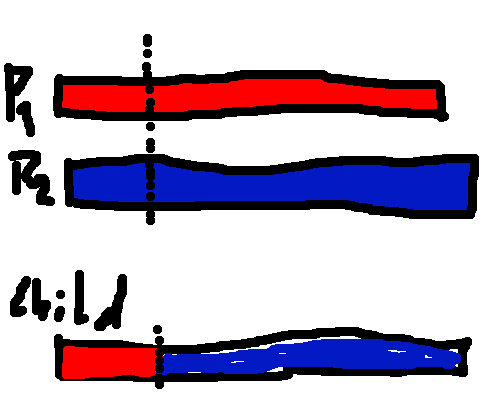
\includegraphics[scale=1.0]{images/Single_Point_Crossover.png}

\subsubsection*{N-Point Crossover}
Der N-Point Crossover ist eine Generallisierung des Single Point Crossovers.
Es werden $n$ Crossover Points entlang der Länge der Eltern gewählt.
Anhand dieser Crossover Points werden die Eltern in $n+1$ Segmente unterteilt.
Das Kind erhält alle Segmente mit geradem Index vom ersten Elternteil und alle Segmente mit 
ungeradem Index vom zweiten Elternteil.
Im Allgemeinen führen mehr cutpoints jedoch zu einer geringeren Effizienz 
des genetischen Algorithmus.~\cite*{TerminologiesAndOperators}

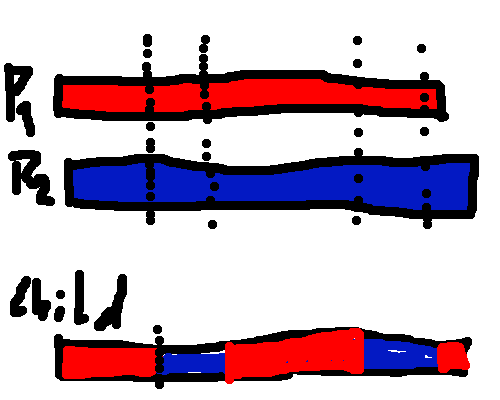
\includegraphics[scale=1.0]{images/N_Point_Crossover.png}

\subsubsection*{Uniform Crossover}
Bei einem uniformen Crossover wird eine Crossovermaske $m$ mit gleicher Länge zu den Eltern erstellt.
Das Kind erhält Gene der Eltern nach dieser Crossover Maske, wobei
$m_i$ angibt, von welchem Elternteil das $i$-te Gen bezogen wird.
Für jedes Elternpaar wird eine neue Crossovermaske erstellt. 
Typischerweise gilt $P(m_i = 1) = P(m_1 = 0) = 0.5$. Die Wahrscheinlichkeit, dass
ein Gen von einem Elternteil bezogen wird kann jedoch auch gewichtet werden anhand 
der Fitness oder Ränge, so dass
$P(m_i = 0) = w$ und $P(m_i = 1) = 1 - w$

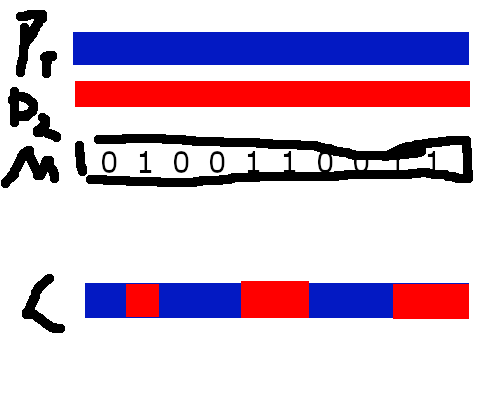
\includegraphics[scale=1.0]{images/Uniform_Crossover.png}

\subsection{Mutationsoperator}
Der Crossoverschritt verringert unweigerlich die genetische Diversität der Population.
Um dem entgegenzuwirken muss es einen Mechanismus geben, welcher neues genetisches Material 
hinzufügt. Dieser Mechanismus ist die Mutation, welche ein Chromosom zufällig verändert.


TODO: Include Examples for Real valued GA crossover 

\subsubsection*{Mutationschance}
Die Mutationschance bestimmt wie viele Gene eines Chromosoms durch die Mutation verändert werden und wie viele
Unverändert bleiben. Bei einer Mutationschance von 100\% werden alle Gene eines Chromosoms verändert 
und der genetische Algorithmus ist equivalent zu einer zufälligen Suche.~\cite*{TerminologiesAndOperators}

\subsection{Ersetzen}
TODO: Ersetzen moped schmoped

\subsection{Ablauf eines genetischen Algorithmus}

Ein Iterationsschritt des klassischen genetischen Algorithmu besteht aus 
Vier Schritten. Die Abbruchbedingung eines Genetischen Algorithmus kann zum Beispiel 
vom Mittelwert, der Summe oder dem Maximalwert der Fitness abhängen oder aber auch einfach 
nach einer vorher festgelegten Anzahl an Iterationen terminieren.
Der Ablauf einer Iteration ist in Grafik so und so beschrieben.

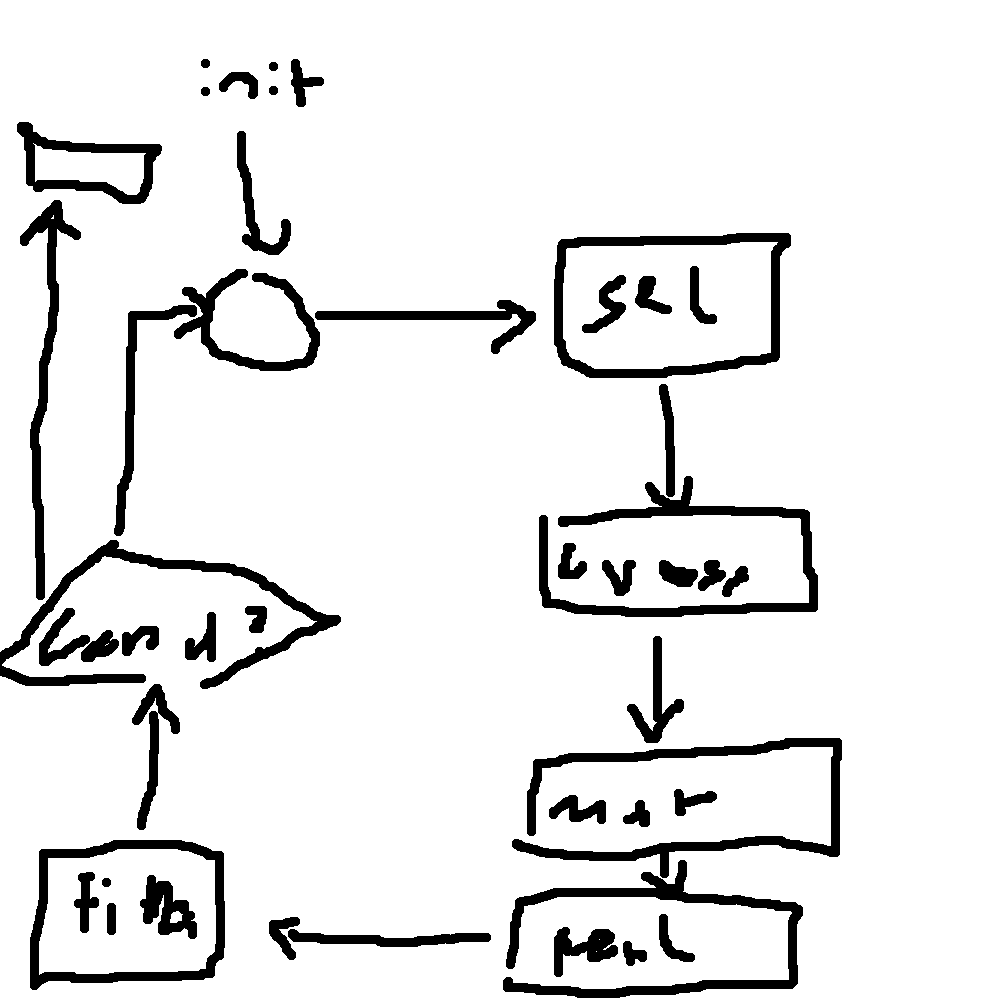
\includegraphics[scale=1.0]{images/Genetic_Algorithm_Flowchart.png}



Population Size
Wählt man diese Zu gering kann es zu einer verfrühten Konvergenz und somit auch einer schlechten Lösung kommen
Gleichzeitig ist die Population size ein Maßgebender Faktor in der Rechenzeit und eine zu große Population könnte 
Rechenzeit verschwenden [GAs]




Im folgenden werde ich bekannte implementationen der genetischen Operatoren eingehen und beschreiben worauf man bei der implementation achten muss

\subsection*{Mutationsoperatoren}
Random Uniform Mutation:
Random Unifor mutation 


\subsection*{Parameter eines genetischen Algorithmus}
- Welche Crossover Funktion (evtl. Parameter der Crossover Funktion)
- Welche Mutations Funktion (evtl. Parameter der Mutations Funktion)
- Populationsgröße
- Rekombination
- Selektionsfunktion
- 

- Populationsgröße
Die globale Suchkapazität eines genetischen Algorithmus hängt stark von
der gewählten Populationsgröße ab. Eine größere Population ist hier von Vorteil.
Jedoch benötigt eine große Population auch mehr Rechenleistung, Speicher und Zeit.~\cite*{TerminologiesAndOperators}

- Auswahl des Mutationsoperators.
Mutationsoperatoren unterscheiden sich stark in der benötigten Rechenleistung.
Der Single Point Crossover-Operator benötigt zum Beispiel nur ein einziges Zufallsereignis, wohingegen
ein Uniformer Crossover-Operator so viele Zufallsereignisse wie es Gene gibt benötigt.
Bei einer Chromosomrepresentation mit vielen Genen macht sich dieser Unterschied bemerkbar.
